\documentclass[orientation=landscape]{tikzposter} % See Section 3

\geometry{paperwidth=48in,paperheight=36in}
\makeatletter
\setlength{\TP@visibletextwidth}{\textwidth-2\TP@innermargin}
\setlength{\TP@visibletextheight}{\textheight-2\TP@innermargin}
\makeatother

\usepackage{amsmath,amsthm, amssymb, latexsym}
\usepackage{algpseudocode,algorithm,algorithmicx}

\newcommand*\Let[2]{\State #1 $\gets$ #2}




\title{\parbox{\linewidth}{\centering On Modifications to Laguerre's Method and the Polynomial Eigenvalue Problem}}
\institute{Davidson College \& DiscoverOrg LLC.}
\author{Thomas R. Cameron \& Nikolas I. Steckley}
%\titlegraphic{Logo}
\usetheme{Rays} % See Section 5
\usebackgroundstyle{Default}
%\usecolorstyle[colorPalette=GreenGrayViolet]{Australia}
\usetitlestyle{Default}
\begin{document}
	\maketitle % See Section 4.1
	\block{Abstract}{Laguerre's method has long been recognized for its strong virtues when computing the roots of a polynomial. Over the years, many modifications to Laguerre's method have been suggested in an attempt to improve its convergence rate and to avoid multiple convergence to a simple root. Now, we present a modification to Laguerre's method for the simultaneous convergence of all roots of a polynomial. Multiple numerical experiments verify both the accuracy and efficiency of this algorithm, and we provide comparisons to other root finding methods, such as POLZEROS and AMVW. Furthermore, we are able to apply this method to the polynomial eigenvalue problem, where it is effective for large degree problems, and the Tridiagonal problem.} % See Section 4.2
	\begin{columns} % See Section 4.4
		\column{0.333} % See Section 4.4
		\block{Introduction}{
			Let $p(\lambda)$ be a polynomial of degree $m$. Let $(z_{1}^{(k)},\ldots,z_{m}^{(k)})$ be approximations to the roots, $r_{1},\ldots,r_{m}$, of $p(\lambda)$ after $k$ iterations. For $1\leq j\leq m$, we define
			\begin{equation}
			\begin{split}
			G_{(j,k)}(\lambda)&=\frac{p^{'}(\lambda)}{p(\lambda)}-\sum_{\substack{i=1\\i\neq j}}^{m}\frac{1}{\lambda-z_{i}^{(k)}}, \\
			H_{(j,k)}(\lambda)&=-\left(\frac{p^{'}(\lambda)}{p(\lambda)}\right)^{'}-\sum_{\substack{i=1\\i\neq j}}^{m}\frac{1}{(\lambda-z_{i}^{(k)})^{2}}.
			\end{split}
			\end{equation}
			Then our next approximation is defined by
			\begin{equation}\label{eq:lag2}
			z_{j}^{(k+1)}=z_{j}^{(k)}-L_{m}(z_{j}^{(k)})
			\end{equation}
			where
			\begin{equation}
			L_{m}(z_{j}^{(k)})=\frac{m}{G_{(j,k)}(z_{j}^{(k)})\pm\sqrt{(m-1)(mH_{(j,k)}(z_{j}^{(k)})-G_{(j,k)}^{2}(z_{j}^{(k)}))}}
			\end{equation}
			and the $\pm$ is chosen to maximize the magnitude of the denominator. 
			}
		\block{Modified Laguerre's Method}{
		\begin{algorithmic}[1]
		\For {$k=1 \textrm{ to } itmax$}
		\For {$j=1 \textrm{ to } m$}
		\If{$j$th approximation has not already converged}
			\Let{$z_{j}$}{$z_{j}-L_{m}(z_{j})$}
		\EndIf
		\EndFor
	    \EndFor
		\end{algorithmic}
}	
		\column{0.333}
		\block{Comparisions}{
			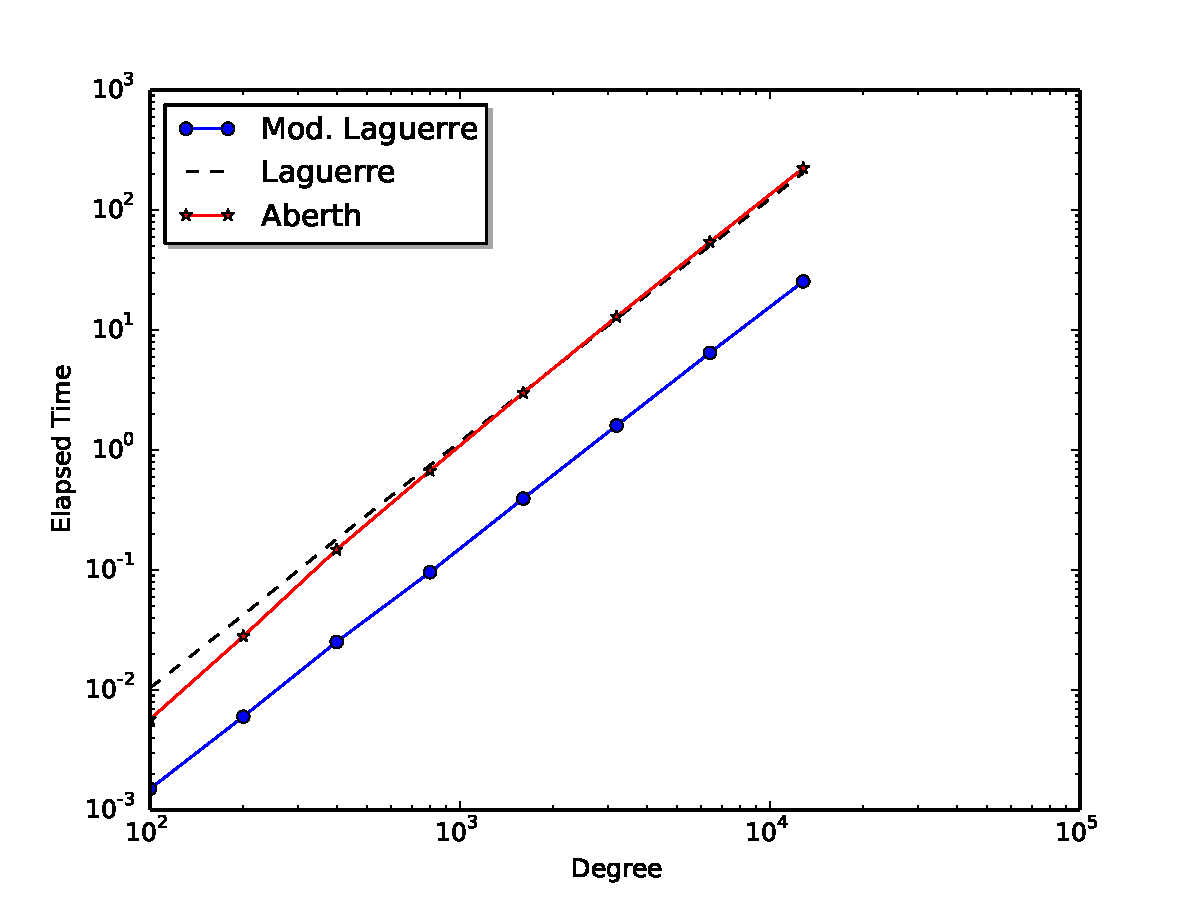
\includegraphics[width=\linewidth]{../develop/tests/diagrams/testMethods}
		}

		\column{0.333}
		\block{Aberth}{
			Let $p(\lambda)$ be a polynomial of degree $m$. Let $(z_{1}^{(k)},\ldots,z_{m}^{(k)})$ be approximations to the roots, $r_{1},\ldots,r_{m}$, of $p(\lambda)$.. For $1\leq j\leq m$, we define
			\begin{equation}
		    A(z_{j})= -\frac{\frac{p(z_{j}^{(k)})}{p^{'}(z_{j}^{(k)})}}{1-\frac{p(z_{j}^{(k)})}{p^{'}(z_{j}^{(k)})} \cdot \sum\limits_{\substack{i=1\\i\neq j}}^{m}\frac{1}{z_{j}^{(k)}-z_{i}^{(k)}}}
			\end{equation}
			The next approximation is then defined by
			\begin{equation}
			z_{j}^{(k+1)}=z_{j}^{(k)}-A(z_{j}^{(k)})
			\end{equation}
		}
		\block{Classical Laguerre}{
			Let $p(\lambda)$ be a polynomial of degree $m$. Let $(z_{1}^{(k)},\ldots,z_{m}^{(k)})$ be approximations to the roots, $r_{1},\ldots,r_{m}$, of $p(\lambda)$. For $1\leq j\leq m$, we define
			\begin{equation}
			\begin{split}
			G_{j}(z_{j}^{(k)})&=\frac{p^{'}(z_{j}^{(k)})}{p(z_{j}^{(k)})}, \\
			H_{j}(z_{j}^{(k)})&=G^{2}_{j}(z_{j}^{(k)})-\frac{p^{''}(z_{j}^{(k)})}{p(z_{j}^{(k)})}.
			\end{split}
			\end{equation}
			Then our next approximation is defined by
			\begin{equation}\label{eq:lag2}
			z_{j}^{(k+1)}=z_{j}^{(k)}-L(z_{j}^{(k)})
			\end{equation}
			where
			\begin{equation}
			L(z_{j}^{(k)})=\frac{m}{G_{j}^{(k)}(z_{j}^{(k)})\pm\sqrt{(m-1)(mH_{j}(z_{j}^{(k)})-G_{j}^{2}(z_{j}^{(k)}))}}
			\end{equation}
			and the $\pm$ is chosen to maximize the magnitude of the denominator. }
		%\note{Notetext} % See Section 4.3
	\end{columns}
\end{document}